\documentclass[11pt,a4paper]{article}
\usepackage[utf8]{inputenc}
\usepackage[T1]{fontenc}
\usepackage[margin=0.7in]{geometry}
\usepackage{hyperref}
\usepackage{booktabs}
\usepackage{enumitem}
\usepackage{tikz}
\usepackage{float}

\usetikzlibrary{shapes.geometric, arrows, positioning}

\hypersetup{colorlinks=true, linkcolor=blue, urlcolor=cyan}
\setlength{\parskip}{0.2em}
\setlength{\parindent}{0pt}
\setlist{nosep, leftmargin=*}

\title{\vspace{-1.5cm}\textbf{Project Plan: Agentic Workflow for Automated Binary/APK Analysis}\vspace{-0.3cm}}
\author{Abdeljalil Otman \quad \small AI Applications in Cybersecurity}
\date{January 25, 2026}

\begin{document}
\maketitle

\section{Project Information}
\begin{itemize}
    \item \textbf{Project Number:} 1 — Agentic Workflow for Automated Binary/APK Analysis
    \item \textbf{Focus:} Binary Executable Analysis (primary), APK Analysis (secondary)
    \item \textbf{Team:} Abdeljalil Otman (Solo Developer)
    \item \textbf{GitHub:} \url{https://github.com/AbdeljalilOtman/agentic-binary-analysis}
\end{itemize}

\section{Methodology}

\subsection{High-Level Approach}
The system uses an LLM-based agent (Agno framework) to orchestrate specialized analysis tools implemented as MCP servers via FastMCP. \textbf{Key principles:} (1) High-level tool abstractions instead of raw command wrappers, (2) Standardized MCP communication, (3) Iterative analysis with agent reasoning.

\subsection{System Architecture}
\begin{figure}[H]
\centering
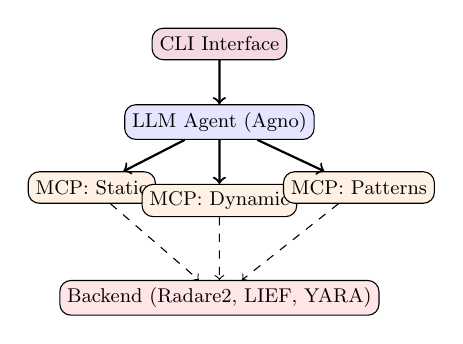
\begin{tikzpicture}[node distance=0.7cm, scale=0.8, transform shape,
    box/.style={rectangle, draw, rounded corners, minimum width=2cm, minimum height=0.5cm, align=center, font=\small}]
\node[box, fill=purple!15] (ui) {CLI Interface};
\node[box, fill=blue!10, below=of ui] (agent) {LLM Agent (Agno)};
\node[box, fill=orange!10, below left=0.5cm and -0.5cm of agent] (mcp1) {MCP: Static};
\node[box, fill=orange!10, below=of agent] (mcp2) {MCP: Dynamic};
\node[box, fill=orange!10, below right=0.5cm and -0.5cm of agent] (mcp3) {MCP: Patterns};
\node[box, fill=red!10, below=1cm of mcp2] (backend) {Backend (Radare2, LIEF, YARA)};
\draw[->, thick] (ui) -- (agent);
\draw[->, thick] (agent) -- (mcp1);
\draw[->, thick] (agent) -- (mcp2);
\draw[->, thick] (agent) -- (mcp3);
\draw[->, dashed] (mcp1) -- (backend);
\draw[->, dashed] (mcp2) -- (backend);
\draw[->, dashed] (mcp3) -- (backend);
\end{tikzpicture}
\end{figure}

\subsection{MCP Tools (FastMCP)}
\begin{itemize}
    \item \textbf{Static Analysis:} \texttt{extract\_crypto\_constants()}, \texttt{extract\_strings\_with\_context()}, \texttt{analyze\_imports\_exports()}
    \item \textbf{Dynamic Analysis:} \texttt{find\_suspicious\_syscalls()}, \texttt{detect\_anti\_analysis()}, \texttt{trace\_data\_flow()}
    \item \textbf{Pattern Detection:} \texttt{analyze\_control\_flow\_anomalies()}, \texttt{detect\_packing\_encryption()}, \texttt{match\_malware\_signatures()}
\end{itemize}

\subsection{Technology Stack}
\begin{tabular}{@{}llll@{}}
\textbf{Agent:} Agno & \textbf{MCP:} FastMCP & \textbf{LLM:} OpenRouter (free tier) & \textbf{Language:} Python 3.11+ \\
\textbf{Binary Analysis:} Radare2, LIEF, Capstone & \textbf{Signatures:} YARA & & \\
\end{tabular}

\section{Implementation Plan}

\subsection{Timeline (8 Weeks: Jan 25 – Mar 22, 2026)}
\begin{tabular}{@{}llp{9cm}@{}}
\toprule
\textbf{Phase} & \textbf{Weeks} & \textbf{Key Tasks} \\
\midrule
1. Foundation & 1–2 & Environment setup, FastMCP structure, basic Agno agent, CLI \\
2. Tool Development & 3–5 & Implement all MCP tools (static, dynamic, pattern detection), unit tests \\
3. Agent Integration & 5–6 & Prompt engineering, tool orchestration, report generation \\
4. Evaluation & 7–8 & Testing with malware samples, documentation, demo preparation \\
\bottomrule
\end{tabular}

\subsection{Milestones}
\textbf{M1 (Week 2):} Basic framework working \quad \textbf{M2 (Week 5):} All tools implemented \quad \textbf{M3 (Week 6):} Integrated agent \quad \textbf{M4 (Week 8):} Final submission

\subsection{Risk Mitigation}
\begin{tabular}{@{}lll@{}}
\toprule
\textbf{Risk} & \textbf{Prob.} & \textbf{Mitigation} \\
\midrule
LLM API rate limits & Medium & Use OpenRouter free tier with low-token prompts \\
Tool integration issues & Medium & Modular design, start with simpler tools \\
Binary analysis accuracy & High & Extensive testing, fallback mechanisms \\
\bottomrule
\end{tabular}

\section{Deliverables}
\begin{enumerate}
    \item \textbf{Software:} Complete agentic analysis system with MCP tools, CLI interface, Docker container
    \item \textbf{Documentation:} README, API docs, architecture guide, usage examples
    \item \textbf{Demo:} Video demonstration + live presentation
\end{enumerate}

\end{document}
